% Created by tikzDevice version 0.12.3.1 on 2023-02-19 11:28:31
% !TEX encoding = UTF-8 Unicode
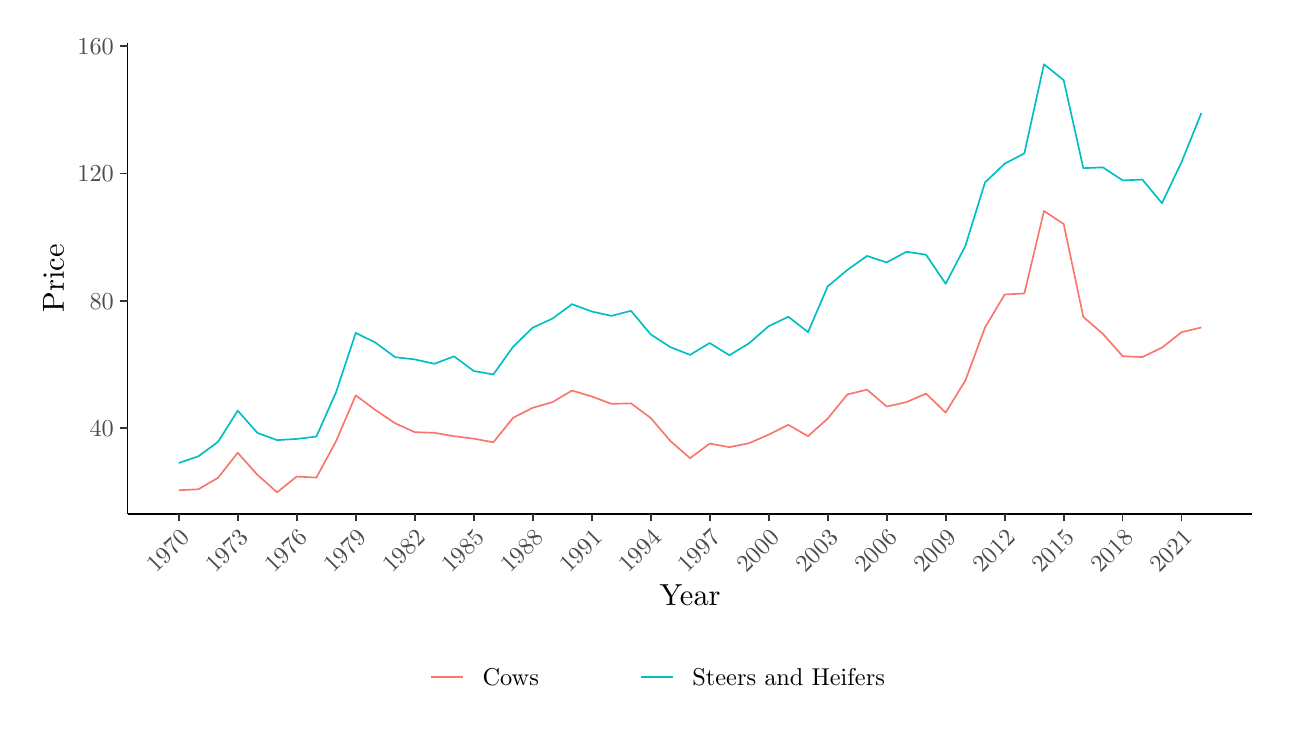
\begin{tikzpicture}[x=1pt,y=1pt]
\definecolor{fillColor}{RGB}{255,255,255}
\path[use as bounding box,fill=fillColor,fill opacity=0.00] (0,0) rectangle (448.07,252.94);
\begin{scope}
\path[clip] (  0.00,  0.00) rectangle (448.07,252.94);
\definecolor{drawColor}{RGB}{255,255,255}
\definecolor{fillColor}{RGB}{255,255,255}

\path[draw=drawColor,line width= 0.6pt,line join=round,line cap=round,fill=fillColor] (  0.00,  0.00) rectangle (448.07,252.94);
\end{scope}
\begin{scope}
\path[clip] ( 36.11, 77.31) rectangle (442.57,247.44);
\definecolor{fillColor}{RGB}{255,255,255}

\path[fill=fillColor] ( 36.11, 77.31) rectangle (442.57,247.44);
\definecolor{drawColor}{RGB}{0,191,196}

\path[draw=drawColor,line width= 0.6pt,line join=round] ( 54.59, 95.64) --
	( 61.69, 98.06) --
	( 68.80,103.28) --
	( 75.90,114.54) --
	( 83.01,106.52) --
	( 90.12,103.89) --
	( 97.22,104.33) --
	(104.33,105.20) --
	(111.43,121.19) --
	(118.54,142.64) --
	(125.65,139.15) --
	(132.75,133.88) --
	(139.86,133.07) --
	(146.96,131.48) --
	(154.07,134.17) --
	(161.18,128.88) --
	(168.28,127.63) --
	(175.39,137.61) --
	(182.49,144.53) --
	(189.60,147.80) --
	(196.71,153.02) --
	(203.81,150.38) --
	(210.92,148.80) --
	(218.02,150.61) --
	(225.13,142.11) --
	(232.24,137.50) --
	(239.34,134.70) --
	(246.45,138.99) --
	(253.55,134.57) --
	(260.66,138.88) --
	(267.77,145.07) --
	(274.87,148.48) --
	(281.98,142.91) --
	(289.08,159.44) --
	(296.19,165.39) --
	(303.30,170.45) --
	(310.40,168.11) --
	(317.51,171.95) --
	(324.61,170.90) --
	(331.72,160.39) --
	(338.83,174.07) --
	(345.93,196.99) --
	(353.04,203.79) --
	(360.14,207.52) --
	(367.25,239.71) --
	(374.36,233.96) --
	(381.46,202.17) --
	(388.57,202.45) --
	(395.67,197.75) --
	(402.78,198.04) --
	(409.89,189.52) --
	(416.99,204.47) --
	(424.10,222.09);
\definecolor{drawColor}{RGB}{248,118,109}

\path[draw=drawColor,line width= 0.6pt,line join=round] ( 54.59, 85.79) --
	( 61.69, 86.14) --
	( 68.80, 90.29) --
	( 75.90, 99.34) --
	( 83.01, 91.36) --
	( 90.12, 85.04) --
	( 97.22, 90.73) --
	(104.33, 90.37) --
	(111.43,103.50) --
	(118.54,120.08) --
	(125.65,114.79) --
	(132.75,110.00) --
	(139.86,106.78) --
	(146.96,106.54) --
	(154.07,105.32) --
	(161.18,104.42) --
	(168.28,103.12) --
	(175.39,111.96) --
	(182.49,115.58) --
	(189.60,117.61) --
	(196.71,121.81) --
	(203.81,119.69) --
	(210.92,117.00) --
	(218.02,117.18) --
	(225.13,111.90) --
	(232.24,103.58) --
	(239.34, 97.37) --
	(246.45,102.64) --
	(253.55,101.36) --
	(260.66,102.79) --
	(267.77,105.89) --
	(274.87,109.43) --
	(281.98,105.32) --
	(289.08,111.69) --
	(296.19,120.41) --
	(303.30,122.15) --
	(310.40,116.03) --
	(317.51,117.62) --
	(324.61,120.70) --
	(331.72,113.86) --
	(338.83,125.45) --
	(345.93,144.59) --
	(353.04,156.53) --
	(360.14,156.90) --
	(367.25,186.71) --
	(374.36,181.98) --
	(381.46,148.39) --
	(388.57,142.26) --
	(395.67,134.22) --
	(402.78,133.91) --
	(409.89,137.33) --
	(416.99,142.92) --
	(424.10,144.61);
\end{scope}
\begin{scope}
\path[clip] (  0.00,  0.00) rectangle (448.07,252.94);
\definecolor{drawColor}{RGB}{0,0,0}

\path[draw=drawColor,line width= 0.6pt,line join=round] ( 36.11, 77.31) --
	( 36.11,247.44);
\end{scope}
\begin{scope}
\path[clip] (  0.00,  0.00) rectangle (448.07,252.94);
\definecolor{drawColor}{gray}{0.30}

\node[text=drawColor,anchor=base east,inner sep=0pt, outer sep=0pt, scale=  0.88] at ( 31.16,105.25) {40};

\node[text=drawColor,anchor=base east,inner sep=0pt, outer sep=0pt, scale=  0.88] at ( 31.16,151.23) {80};

\node[text=drawColor,anchor=base east,inner sep=0pt, outer sep=0pt, scale=  0.88] at ( 31.16,197.22) {120};

\node[text=drawColor,anchor=base east,inner sep=0pt, outer sep=0pt, scale=  0.88] at ( 31.16,243.20) {160};
\end{scope}
\begin{scope}
\path[clip] (  0.00,  0.00) rectangle (448.07,252.94);
\definecolor{drawColor}{gray}{0.20}

\path[draw=drawColor,line width= 0.6pt,line join=round] ( 33.36,108.28) --
	( 36.11,108.28);

\path[draw=drawColor,line width= 0.6pt,line join=round] ( 33.36,154.27) --
	( 36.11,154.27);

\path[draw=drawColor,line width= 0.6pt,line join=round] ( 33.36,200.25) --
	( 36.11,200.25);

\path[draw=drawColor,line width= 0.6pt,line join=round] ( 33.36,246.23) --
	( 36.11,246.23);
\end{scope}
\begin{scope}
\path[clip] (  0.00,  0.00) rectangle (448.07,252.94);
\definecolor{drawColor}{RGB}{0,0,0}

\path[draw=drawColor,line width= 0.6pt,line join=round] ( 36.11, 77.31) --
	(442.57, 77.31);
\end{scope}
\begin{scope}
\path[clip] (  0.00,  0.00) rectangle (448.07,252.94);
\definecolor{drawColor}{gray}{0.20}

\path[draw=drawColor,line width= 0.6pt,line join=round] ( 54.59, 74.56) --
	( 54.59, 77.31);

\path[draw=drawColor,line width= 0.6pt,line join=round] ( 75.90, 74.56) --
	( 75.90, 77.31);

\path[draw=drawColor,line width= 0.6pt,line join=round] ( 97.22, 74.56) --
	( 97.22, 77.31);

\path[draw=drawColor,line width= 0.6pt,line join=round] (118.54, 74.56) --
	(118.54, 77.31);

\path[draw=drawColor,line width= 0.6pt,line join=round] (139.86, 74.56) --
	(139.86, 77.31);

\path[draw=drawColor,line width= 0.6pt,line join=round] (161.18, 74.56) --
	(161.18, 77.31);

\path[draw=drawColor,line width= 0.6pt,line join=round] (182.49, 74.56) --
	(182.49, 77.31);

\path[draw=drawColor,line width= 0.6pt,line join=round] (203.81, 74.56) --
	(203.81, 77.31);

\path[draw=drawColor,line width= 0.6pt,line join=round] (225.13, 74.56) --
	(225.13, 77.31);

\path[draw=drawColor,line width= 0.6pt,line join=round] (246.45, 74.56) --
	(246.45, 77.31);

\path[draw=drawColor,line width= 0.6pt,line join=round] (267.77, 74.56) --
	(267.77, 77.31);

\path[draw=drawColor,line width= 0.6pt,line join=round] (289.08, 74.56) --
	(289.08, 77.31);

\path[draw=drawColor,line width= 0.6pt,line join=round] (310.40, 74.56) --
	(310.40, 77.31);

\path[draw=drawColor,line width= 0.6pt,line join=round] (331.72, 74.56) --
	(331.72, 77.31);

\path[draw=drawColor,line width= 0.6pt,line join=round] (353.04, 74.56) --
	(353.04, 77.31);

\path[draw=drawColor,line width= 0.6pt,line join=round] (374.36, 74.56) --
	(374.36, 77.31);

\path[draw=drawColor,line width= 0.6pt,line join=round] (395.67, 74.56) --
	(395.67, 77.31);

\path[draw=drawColor,line width= 0.6pt,line join=round] (416.99, 74.56) --
	(416.99, 77.31);
\end{scope}
\begin{scope}
\path[clip] (  0.00,  0.00) rectangle (448.07,252.94);
\definecolor{drawColor}{gray}{0.30}

\node[text=drawColor,rotate= 45.00,anchor=base east,inner sep=0pt, outer sep=0pt, scale=  0.88] at ( 58.87, 68.07) {1970};

\node[text=drawColor,rotate= 45.00,anchor=base east,inner sep=0pt, outer sep=0pt, scale=  0.88] at ( 80.19, 68.07) {1973};

\node[text=drawColor,rotate= 45.00,anchor=base east,inner sep=0pt, outer sep=0pt, scale=  0.88] at (101.51, 68.07) {1976};

\node[text=drawColor,rotate= 45.00,anchor=base east,inner sep=0pt, outer sep=0pt, scale=  0.88] at (122.83, 68.07) {1979};

\node[text=drawColor,rotate= 45.00,anchor=base east,inner sep=0pt, outer sep=0pt, scale=  0.88] at (144.14, 68.07) {1982};

\node[text=drawColor,rotate= 45.00,anchor=base east,inner sep=0pt, outer sep=0pt, scale=  0.88] at (165.46, 68.07) {1985};

\node[text=drawColor,rotate= 45.00,anchor=base east,inner sep=0pt, outer sep=0pt, scale=  0.88] at (186.78, 68.07) {1988};

\node[text=drawColor,rotate= 45.00,anchor=base east,inner sep=0pt, outer sep=0pt, scale=  0.88] at (208.10, 68.07) {1991};

\node[text=drawColor,rotate= 45.00,anchor=base east,inner sep=0pt, outer sep=0pt, scale=  0.88] at (229.42, 68.07) {1994};

\node[text=drawColor,rotate= 45.00,anchor=base east,inner sep=0pt, outer sep=0pt, scale=  0.88] at (250.73, 68.07) {1997};

\node[text=drawColor,rotate= 45.00,anchor=base east,inner sep=0pt, outer sep=0pt, scale=  0.88] at (272.05, 68.07) {2000};

\node[text=drawColor,rotate= 45.00,anchor=base east,inner sep=0pt, outer sep=0pt, scale=  0.88] at (293.37, 68.07) {2003};

\node[text=drawColor,rotate= 45.00,anchor=base east,inner sep=0pt, outer sep=0pt, scale=  0.88] at (314.69, 68.07) {2006};

\node[text=drawColor,rotate= 45.00,anchor=base east,inner sep=0pt, outer sep=0pt, scale=  0.88] at (336.01, 68.07) {2009};

\node[text=drawColor,rotate= 45.00,anchor=base east,inner sep=0pt, outer sep=0pt, scale=  0.88] at (357.32, 68.07) {2012};

\node[text=drawColor,rotate= 45.00,anchor=base east,inner sep=0pt, outer sep=0pt, scale=  0.88] at (378.64, 68.07) {2015};

\node[text=drawColor,rotate= 45.00,anchor=base east,inner sep=0pt, outer sep=0pt, scale=  0.88] at (399.96, 68.07) {2018};

\node[text=drawColor,rotate= 45.00,anchor=base east,inner sep=0pt, outer sep=0pt, scale=  0.88] at (421.28, 68.07) {2021};
\end{scope}
\begin{scope}
\path[clip] (  0.00,  0.00) rectangle (448.07,252.94);
\definecolor{drawColor}{RGB}{0,0,0}

\node[text=drawColor,anchor=base,inner sep=0pt, outer sep=0pt, scale=  1.10] at (239.34, 44.09) {Year};
\end{scope}
\begin{scope}
\path[clip] (  0.00,  0.00) rectangle (448.07,252.94);
\definecolor{drawColor}{RGB}{0,0,0}

\node[text=drawColor,rotate= 90.00,anchor=base,inner sep=0pt, outer sep=0pt, scale=  1.10] at ( 13.08,162.38) {Price};
\end{scope}
\begin{scope}
\path[clip] (  0.00,  0.00) rectangle (448.07,252.94);
\definecolor{fillColor}{RGB}{255,255,255}

\path[fill=fillColor] (133.45,  5.50) rectangle (345.24, 30.95);
\end{scope}
\begin{scope}
\path[clip] (  0.00,  0.00) rectangle (448.07,252.94);
\definecolor{drawColor}{RGB}{248,118,109}

\path[draw=drawColor,line width= 0.6pt,line join=round] (145.89, 18.23) -- (157.45, 18.23);
\end{scope}
\begin{scope}
\path[clip] (  0.00,  0.00) rectangle (448.07,252.94);
\definecolor{drawColor}{RGB}{248,118,109}

\path[draw=drawColor,line width= 0.6pt,line join=round] (145.89, 18.23) -- (157.45, 18.23);
\end{scope}
\begin{scope}
\path[clip] (  0.00,  0.00) rectangle (448.07,252.94);
\definecolor{drawColor}{RGB}{0,191,196}

\path[draw=drawColor,line width= 0.6pt,line join=round] (221.68, 18.23) -- (233.24, 18.23);
\end{scope}
\begin{scope}
\path[clip] (  0.00,  0.00) rectangle (448.07,252.94);
\definecolor{drawColor}{RGB}{0,191,196}

\path[draw=drawColor,line width= 0.6pt,line join=round] (221.68, 18.23) -- (233.24, 18.23);
\end{scope}
\begin{scope}
\path[clip] (  0.00,  0.00) rectangle (448.07,252.94);
\definecolor{drawColor}{RGB}{0,0,0}

\node[text=drawColor,anchor=base west,inner sep=0pt, outer sep=0pt, scale=  0.88] at (164.40, 15.20) {Cows};
\end{scope}
\begin{scope}
\path[clip] (  0.00,  0.00) rectangle (448.07,252.94);
\definecolor{drawColor}{RGB}{0,0,0}

\node[text=drawColor,anchor=base west,inner sep=0pt, outer sep=0pt, scale=  0.88] at (240.19, 15.20) {Steers and Heifers};
\end{scope}
\end{tikzpicture}
